\documentclass{beamer}
\usetheme{Madrid}
\usecolortheme{dolphin}
\usepackage{tikz}
\usepackage{amsmath}
\usepackage{amssymb}


\usetikzlibrary{shapes,arrows,positioning,fit,calc,decorations.pathreplacing,decorations.markings}
\usepackage{amsmath}

\title{Introduction to Propositional Logic}
\author{Brendan Shea, PhD}

\begin{document}

\begin{frame}
\titlepage
\end{frame}

\begin{frame}
\frametitle{What is Propositional Logic?}
\begin{itemize}
    \item \textbf{Propositional logic} is a branch of logic that studies how simple statements combine to form complex statements.
    \item Propositional logic helps us determine whether arguments are valid based on their structure alone.
    \item We use symbols to represent statements and show how they connect to each other.
    \item Propositional logic is the foundation for mathematical proofs, computer programming, and clear reasoning.
\end{itemize}

\begin{alertblock}{Why Study Logic?}
    Logic gives us tools to evaluate arguments, avoid fallacies, and communicate precisely in mathematics, computer science, law, and everyday reasoning.
\end{alertblock}
\end{frame}

\begin{frame}
\frametitle{Statements vs. Non-Statements}
\begin{itemize}
    \item A \textbf{statement} (or proposition) is a declarative sentence that is either true or false, but not both.
    \item Statements make claims about the world that can be evaluated as true or false.
    \item Questions, commands, exclamations, and opinions are not statements in propositional logic.
    \item We use letters like $p$, $q$, and $r$ to represent simple statements.
\end{itemize}

\begin{block}{Examples}
\begin{tabular}{ll}
\textbf{Statements} & \textbf{Non-Statements} \\
\hline
Paris is in France. & Is Paris in France? \\
2 + 2 = 5. & Go to Paris! \\
All squares are rectangles. & I wish I were in Paris. \\
\end{tabular}
\end{block}
\end{frame}

\begin{frame}
\frametitle{Introducing Logical Symbols}
\begin{itemize}
    \item \textbf{Logical symbols} allow us to write complex statements in a precise, mathematical way.
    \item Each symbol represents a specific logical operation or connection between statements.
    \item Using symbols helps us avoid the ambiguity that can occur in everyday language.
    \item We combine symbols to translate complex English sentences into logical form.
\end{itemize}

\begin{center}
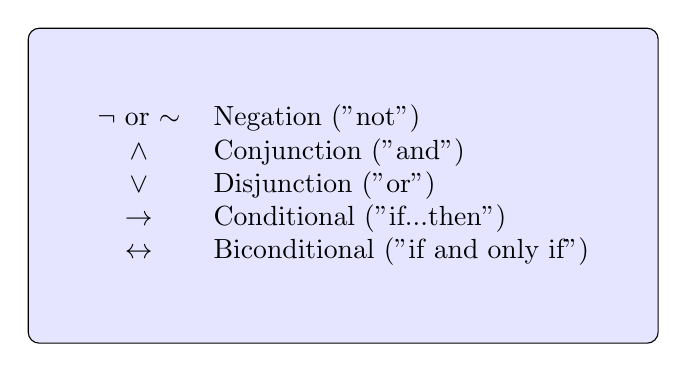
\begin{tikzpicture}
\node[draw, rectangle, rounded corners, fill=blue!10, minimum width=8cm, minimum height=4cm] {
\begin{tabular}{cl}
$\neg$ or $\sim$ & Negation ("not") \\
$\wedge$ & Conjunction ("and") \\
$\vee$ & Disjunction ("or") \\
$\rightarrow$ & Conditional ("if...then") \\
$\leftrightarrow$ & Biconditional ("if and only if") \\
\end{tabular}
};
\end{tikzpicture}
\end{center}
\end{frame}


\begin{frame}
    \frametitle{The Negation Symbol ($\sim$): Saying "Not"}
    \begin{itemize}
        \item \textbf{Negation} is the simplest logical operation, which simply reverses the truth value of a statement.
        \item We write the negation of statement $p$ as $\sim p$ (read as "not p").
        \item If $p$ is true, then $\sim p$ is false; if $p$ is false, then $\sim p$ is true.
        \item Double negation cancels out: $\sim(\sim p)$ is equivalent to $p$.
    \end{itemize}
    
    \begin{example}
    Let $p$ = "It is raining."\\
    $\sim p$ = "It is not raining."\\
    Let $q$ = "The earth is flat."\\
    $\sim q$ = "The earth is not flat."
    \end{example}
    \end{frame}
    
    \begin{frame}
    \frametitle{The Conjunction Symbol ($\wedge$): Saying "And"}
    \begin{itemize}
        \item \textbf{Conjunction} connects two statements with "and," requiring both to be true.
        \item We write the conjunction of statements $p$ and $q$ as $p \wedge q$ (read as "p and q").
        \item $p \wedge q$ is true only when both $p$ and $q$ are true.
        \item $p \wedge q$ is false if either $p$ is false, $q$ is false, or both are false.
    \end{itemize}
    
    \begin{block}{Real-World Example}
    To get an A in this class, you need to pass the midterm exam AND complete the final project.\\
    Let $p$ = "You pass the midterm exam."\\
    Let $q$ = "You complete the final project."\\
    Getting an A = $p \wedge q$
    \end{block}
    \end{frame}
    
    \begin{frame}
    \frametitle{The Disjunction Symbol ($\vee$): Saying "Or"}
    \begin{itemize}
        \item \textbf{Disjunction} connects two statements with "or," requiring at least one to be true.
        \item We write the disjunction of statements $p$ and $q$ as $p \vee q$ (read as "p or q").
        \item $p \vee q$ is true when $p$ is true, $q$ is true, or both are true.
        \item $p \vee q$ is false only when both $p$ and $q$ are false.
    \end{itemize}
    
    \begin{alertblock}{Important Note}
    In logic, we use the \textbf{inclusive or} by default, which means "$p$ or $q$ or both."
    This is different from the \textbf{exclusive or} (sometimes called "either/or"), which means "$p$ or $q$ but not both."
    \end{alertblock}
    \end{frame}
    
    \begin{frame}
    \frametitle{The Conditional Symbol ($\rightarrow$): "If...Then"}
    \begin{itemize}
        \item A \textbf{conditional statement} expresses that one thing depends on another.
        \item We write "if $p$ then $q$" as $p \rightarrow q$ (read as "p implies q").
        \item The statement $p$ is called the \textbf{antecedent}, and $q$ is called the \textbf{consequent}.
        \item $p \rightarrow q$ is false only when $p$ is true and $q$ is false; it is true in all other cases.
    \end{itemize}
    
    \begin{tabular}{|p{0.9\textwidth}|}
    \hline
    If you study hard, then you will pass the test.\\[0.2cm]
    $p$: You study hard (antecedent)\\
    $q$: You will pass the test (consequent)\\
    $p \rightarrow q$: If you study hard, then you will pass the test.\\[0.2cm]
    \textbf{The conditional is only false when} you study hard but do not pass.\\
    \hline
    \end{tabular}
    \end{frame}

    \begin{frame}
        \frametitle{The Biconditional Symbol ($\leftrightarrow$): "If and Only If"}
        \begin{itemize}
            \item A \textbf{biconditional statement} expresses that two statements have the same truth value.
            \item We write "$p$ if and only if $q$" as $p \leftrightarrow q$ (read as "$p$ if and only if $q$").
            \item $p \leftrightarrow q$ is true when both $p$ and $q$ are true, or both are false.
            \item $p \leftrightarrow q$ is false when one statement is true and the other is false.
        \end{itemize}
        
        \begin{block}{Understanding Biconditionals}
        $p \leftrightarrow q$ is equivalent to $(p \rightarrow q) \wedge (q \rightarrow p)$\\
        It means "if $p$ then $q$, AND if $q$ then $p$"\\
        Example: "A triangle is equilateral if and only if all its angles are equal."
        \end{block}
        \end{frame}
        
        \begin{frame}
        \frametitle{Translating English to Symbols: Simple Statements}
        \begin{itemize}
            \item Translating English sentences into logical symbols requires identifying the logical structure.
            \item First, identify simple statements and assign letters like $p$, $q$, $r$ to them.
            \item Then identify logical connectives (and, or, not, if-then, if and only if).
            \item Finally, combine the symbols according to the structure of the original sentence.
        \end{itemize}
        
        \begin{example}
        "It is not raining, but it is cold."\\
        Let $p$ = "It is raining." Let $q$ = "It is cold."\\
        Translation: $\sim p \wedge q$\\[0.3cm]
        "Either I will go to the movie or I will stay home."\\
        Let $r$ = "I will go to the movie." Let $s$ = "I will stay home."\\
        Translation: $r \vee s$
        \end{example}
        \end{frame}
        
        \begin{frame}
        \frametitle{Translating English to Symbols: Complex Statements}
        \begin{itemize}
            \item Complex statements may contain multiple logical connectives.
            \item \textbf{Parentheses} help clarify the order of operations in complex statements.
            \item Work step by step, breaking down complicated sentences into simpler parts.
            \item Be careful with negations, as they can apply to individual statements or entire expressions.
        \end{itemize}
        
        \begin{block}{Example Translation}
        "If it's sunny and warm, then I'll go swimming or hiking."\\[0.2cm]
        Let $p$ = "It's sunny."\\
        Let $q$ = "It's warm."\\
        Let $r$ = "I'll go swimming."\\
        Let $s$ = "I'll go hiking."\\[0.2cm]
        Translation: $(p \wedge q) \rightarrow (r \vee s)$
        \end{block}

        \end{frame}

        \begin{frame}
        \frametitle{Common Phrases for Conditionals}
        \begin{itemize}
            \item Conditionals ($p \rightarrow q$) can be expressed in many different ways in English.
            \item The "if-then" form is just one way to express a conditional relationship.
            \item Understanding these different forms helps translate real-world statements into logic.
            \item The logical meaning remains the same regardless of the phrasing.
        \end{itemize}
        
        \begin{block}{Different Ways to Say $p \rightarrow q$}
            \scriptsize
        \begin{itemize}
            \item If $p$, then $q$.
            \item $p$ implies $q$.
            \item $p$ only if $q$.
            \item $q$ if $p$.
            \item $p$ is sufficient for $q$.
            \item $q$ is necessary for $p$.
            \item Unless not-$q$, $p$.
        \end{itemize}
        \end{block}
        \end{frame}

        \begin{frame}
            \frametitle{The Biconditional Symbol ($\leftrightarrow$): "If and Only If"}
            \begin{itemize}
                \item A \textbf{biconditional statement} expresses that two statements have the same truth value.
                \item We write "$p$ if and only if $q$" as $p \leftrightarrow q$ (read as "$p$ if and only if $q$").
                \item $p \leftrightarrow q$ is true when both $p$ and $q$ are true, or both are false.
                \item $p \leftrightarrow q$ is false when one statement is true and the other is false.
            \end{itemize}
            
            \begin{block}{Understanding Biconditionals}
            $p \leftrightarrow q$ is equivalent to $(p \rightarrow q) \wedge (q \rightarrow p)$\\
            It means "if $p$ then $q$, AND if $q$ then $p$"\\
            Example: "A triangle is equilateral if and only if all its angles are equal."
            \end{block}
            \end{frame}
            
            \begin{frame}
            \frametitle{Translating English to Symbols: Simple Statements}
            \begin{itemize}
                \item Translating English sentences into logical symbols requires identifying the logical structure.
                \item First, identify simple statements and assign letters like $p$, $q$, $r$ to them.
                \item Then identify logical connectives (and, or, not, if-then, if and only if).
                \item Finally, combine the symbols according to the structure of the original sentence.
            \end{itemize}
            
            \begin{example}
            "It is not raining, but it is cold."\\
            Let $p$ = "It is raining." Let $q$ = "It is cold."\\
            Translation: $\sim p \wedge q$\\[0.3cm]
            "Either I will go to the movie or I will stay home."\\
            Let $r$ = "I will go to the movie." Let $s$ = "I will stay home."\\
            Translation: $r \vee s$
            \end{example}
            \end{frame}
            
            \begin{frame}
            \frametitle{Translating English to Symbols: Complex Statements}
            \begin{itemize}
                \item Complex statements may contain multiple logical connectives.
                \item \textbf{Parentheses} help clarify the order of operations in complex statements.
                \item Work step by step, breaking down complicated sentences into simpler parts.
                \item Be careful with negations, as they can apply to individual statements or entire expressions.
            \end{itemize}
            
            \begin{block}{Example Translation}
            "If it's sunny and warm, then I'll go swimming or hiking."\\[0.2cm]
            Let $p$ = "It's sunny."\\
            Let $q$ = "It's warm."\\
            Let $r$ = "I'll go swimming."\\
            Let $s$ = "I'll go hiking."\\[0.2cm]
            Translation: $(p \wedge q) \rightarrow (r \vee s)$
            \end{block}
            \end{frame}
            
            \begin{frame}
            \frametitle{Common Phrases for Conditionals}
            \begin{itemize}
                \item Conditionals ($p \rightarrow q$) can be expressed in many different ways in English.
                \item The "if-then" form is just one way to express a conditional relationship.
                \item Understanding these different forms helps translate real-world statements into logic.
                \item The logical meaning remains the same regardless of the phrasing.
            \end{itemize}
            
            \begin{block}{Different Ways to Say $p \rightarrow q$}
                \scriptsize
            \begin{itemize}
                \item If $p$, then $q$.
                \item $p$ implies $q$.
                \item $p$ only if $q$.
                \item $q$ if $p$.
                \item $p$ is sufficient for $q$.
                \item $q$ is necessary for $p$.
                \item Unless not-$q$, $p$.
            \end{itemize}
            \end{block}
            \end{frame}


            \begin{frame}
                \frametitle{Spotting Hidden Conditionals in Everyday Language}
                \begin{itemize}
                    \item Many English sentences contain \textbf{hidden conditionals} that are not expressed in the "if-then" form.
                    \item Signs, warnings, and rules often contain implicit conditional statements.
                    \item Recognizing these allows us to translate a wider range of statements into logical form.
                    \item Translating these statements correctly is crucial for analyzing arguments.
                \end{itemize}
                
                \begin{alertblock}{Examples of Hidden Conditionals}
                "No pets allowed" $\rightarrow$ "If you have a pet, then you are not allowed."
                
                "Students must complete homework to pass" $\rightarrow$ "If a student does not complete homework, then the student will not pass."
                
                "Only adults may enter" $\rightarrow$ "If a person enters, then that person is an adult."
                \end{alertblock}
                \end{frame}
                
                \begin{frame}
                \frametitle{Truth Values: True or False}
                \begin{itemize}
                    \item In propositional logic, every statement has exactly one \textbf{truth value}: True (T) or False (F).
                    \item The truth value of a complex statement depends on the truth values of its simple components.
                    \item Logical operators ($\sim$, $\wedge$, $\vee$, $\rightarrow$, $\leftrightarrow$) have specific rules for determining truth values.
                    \item These rules are consistent and do not depend on the content of the statements.
                \end{itemize}
                
                \begin{center}
                \begin{tabular}{|p{0.9\textwidth}|}
                \hline
                Statement: "Paris is the capital of France."\\
                Truth value: TRUE\\[0.3cm]
                Statement: "New York is the capital of the United States."\\
                Truth value: FALSE\\[0.3cm]
                Statement: "Paris is the capital of France AND New York is the capital of the United States."\\
                Truth value: FALSE (since one component is false)\\
                \hline
                \end{tabular}
                \end{center}
                \end{frame}
                
                \begin{frame}
                \frametitle{Introduction to Truth Tables}
                \begin{itemize}
                    \item A \textbf{truth table} is a systematic way to determine the truth value of a compound statement.
                    \item Truth tables list all possible combinations of truth values for the simple statements.
                    \item Each row represents one possible scenario of truth values.
                    \item For $n$ simple statements, there are $2^n$ possible combinations of truth values.
                \end{itemize}
                
                \begin{block}{Structure of a Truth Table}
                \begin{itemize}
                    \item Left columns show truth values of simple statements ($p$, $q$, etc.)
                    \item Right columns show truth values of increasingly complex expressions
                    \item Final column shows truth value of the complete expression
                    \item Each row represents one possible "world" or scenario
                \end{itemize}
                \end{block}
                \end{frame}
                
                \begin{frame}
                \frametitle{Truth Table for Negation}
                \begin{itemize}
                    \item The truth table for negation ($\sim p$) shows how negation flips truth values.
                    \item It is the simplest truth table, with only two rows (since there is only one statement, $p$).
                    \item Understanding negation is fundamental to building more complex truth tables.
                    \item We can read the table as: "When $p$ is true, $\sim p$ is false; when $p$ is false, $\sim p$ is true."
                \end{itemize}
                
                \begin{center}
                \begin{tabular}{|c|c|}
                \hline
                $p$ & $\sim p$ \\
                \hline
                T & F \\
                \hline
                F & T \\
                \hline
                \end{tabular}
                \end{center}
                
                \begin{example}
                    \scriptsize
                Let $p$ = "The sun is shining."\\
                If it's true that the sun is shining, then "The sun is not shining" ($\sim p$) is false.\\
                If it's false that the sun is shining, then "The sun is not shining" ($\sim p$) is true.
                \end{example}
                \end{frame}

                \begin{frame}
                    \frametitle{Truth Table for Conjunction}
                    \begin{itemize}
                        \item The truth table for conjunction ($p \wedge q$) shows when two statements joined by "and" are true.
                        \item A conjunction is true only when both of its components (called \textbf{conjuncts}) are true.
                        \item If either component is false, the entire conjunction is false.
                        \item This aligns with our everyday understanding of "and" in statements.
                    \end{itemize}
                    
                    \begin{center}
                        \scriptsize
                    \begin{tabular}{|c|c|c|}
                    \hline
                    $p$ & $q$ & $p \wedge q$ \\
                    \hline
                    T & T & T \\
                    \hline
                    T & F & F \\
                    \hline
                    F & T & F \\
                    \hline
                    F & F & F \\
                    \hline
                    \end{tabular}
                    \end{center}
                    
                    \begin{example}
                    "It is raining and it is cold."\\
                    This statement is true only when both "It is raining" AND "It is cold" are true.
                    \end{example}
                    \end{frame}
                    
                    \begin{frame}
                    \frametitle{Truth Table for Disjunction}
                    \begin{itemize}
                        \item The truth table for disjunction ($p \vee q$) shows when two statements joined by "or" are true.
                        \item A disjunction is true when at least one of its components (called \textbf{disjuncts}) is true.
                        \item A disjunction is false only when both of its components are false.
                        \item Remember that we use the inclusive "or" in logic, meaning "either or both."
                    \end{itemize}
                    
                    \begin{center}
                        \scriptsize
                    \begin{tabular}{|c|c|c|}
                    \hline
                    $p$ & $q$ & $p \vee q$ \\
                    \hline
                    T & T & T \\
                    \hline
                    T & F & T \\
                    \hline
                    F & T & T \\
                    \hline
                    F & F & F \\
                    \hline
                    \end{tabular}
                    \end{center}
                    
                    \begin{block}{Real-World Example}
                    "To apply for this job, you need a college degree or five years of experience."\\
                    You qualify if you have: a degree only, experience only, or both.
                    \end{block}
                    \end{frame}
                    
                    \begin{frame}
                    \frametitle{Truth Table for Conditional}
                    \begin{itemize}
                        \item The truth table for the conditional ($p \rightarrow q$) often seems counterintuitive at first.
                        \item A conditional is false only when the antecedent ($p$) is true and the consequent ($q$) is false.
                        \item A conditional with a false antecedent is always true, regardless of the consequent.
                        \item Think of a conditional as making a promise: it's broken only when the promise isn't fulfilled.
                    \end{itemize}
                    
                    \begin{center}
                        \scriptsize
                    \begin{tabular}{|c|c|c|}
                    \hline
                    $p$ & $q$ & $p \rightarrow q$ \\
                    \hline
                    T & T & T \\
                    \hline
                    T & F & F \\
                    \hline
                    F & T & T \\
                    \hline
                    F & F & T \\
                    \hline
                    \end{tabular}
                    \end{center}
                    
                    \begin{alertblock}{Why Are The Bottom Two Rows True?}
                        \scriptsize
                    If the antecedent ($p$) is false, the conditional is automatically true. This is called a \textbf{vacuously true} conditional. It's like saying, "If I'm the Queen of England, then I'll give you a million dollars." Since I'm not the Queen, the promise can't be broken!
                    \end{alertblock}
                    \end{frame}
                    
                    \begin{frame}
                    \frametitle{Truth Table for Biconditional}
                    \begin{itemize}
                        \scriptsize
                        \item The truth table for the biconditional ($p \leftrightarrow q$) shows when two statements have the same truth value.
                        \item A biconditional is true when both components are true or both components are false.
                        \item A biconditional is false when one component is true and the other is false.
                        \item The biconditional can be thought of as a "double conditional" or "two-way implication."
                    \end{itemize}
                    
                    \begin{center}
                        \scriptsize
                    \begin{tabular}{|c|c|c|}
                    \hline
                    $p$ & $q$ & $p \leftrightarrow q$ \\
                    \hline
                    T & T & T \\
                    \hline
                    T & F & F \\
                    \hline
                    F & T & F \\
                    \hline
                    F & F & T \\
                    \hline
                    \end{tabular}
                    \end{center}
                    
                    \begin{example}
                        \scriptsize
                    "A number is even if and only if it is divisible by 2."\\
                    When a number is even AND divisible by 2: true\\
                    When a number is not even AND not divisible by 2: true\\
                    When a number is even BUT not divisible by 2: false (impossible)\\
                    When a number is not even BUT divisible by 2: false (impossible)
                    \end{example}
                    \end{frame}

                    \begin{frame}
                        \frametitle{Building Complex Truth Tables: Step by Step}
                        \begin{itemize}
                            \item Complex logical expressions require building truth tables in systematic steps.
                            \item Work from the inside out, calculating intermediate expressions before the final result.
                            \item Add columns for each sub-expression to track your work clearly.
                            \item The order of operations in logic: parentheses, negation, conjunction/disjunction, conditional, biconditional.
                        \end{itemize}
                        
                        \begin{example}
                            \scriptsize
                        Truth table for $(p \vee q) \rightarrow \sim r$\\[0.2cm]
                        \begin{tabular}{|c|c|c|c|c|c|}
                        \hline
                        $p$ & $q$ & $r$ & $p \vee q$ & $\sim r$ & $(p \vee q) \rightarrow \sim r$ \\
                        \hline
                        T & T & T & T & F & F \\
                        \hline
                        T & T & F & T & T & T \\
                        \hline
                        T & F & T & T & F & F \\
                        \hline
                        T & F & F & T & T & T \\
                        \hline
                        F & T & T & T & F & F \\
                        \hline
                        F & T & F & T & T & T \\
                        \hline
                        F & F & T & F & F & T \\
                        \hline
                        F & F & F & F & T & T \\
                        \hline
                        \end{tabular}
                        \end{example}
                        \end{frame}
                        
                        \begin{frame}
                        \frametitle{Logical Equivalence: When Statements Mean the Same Thing}
                        \begin{itemize}
                            \item Two statements are \textbf{logically equivalent} if they have identical truth values in all possible scenarios.
                            \item We write "$p$ is logically equivalent to $q$" as $p \equiv q$ (note this is not a logical operator).
                            \item Truth tables can be used to determine if two statements are logically equivalent.
                            \item Recognizing logical equivalences helps simplify complex expressions.
                        \end{itemize}
                        
                        \begin{block}{Important Logical Equivalences}
                            \scriptsize
                        \begin{itemize}
                            \item Double Negation: $\sim(\sim p) \equiv p$
                            \item Commutative Laws: $p \wedge q \equiv q \wedge p$; $p \vee q \equiv q \vee p$
                            \item De Morgan's Laws: $\sim(p \wedge q) \equiv \sim p \vee \sim q$; $\sim(p \vee q) \equiv \sim p \wedge \sim q$
                            \item Conditional Equivalence: $p \rightarrow q \equiv \sim p \vee q$
                        \end{itemize}
                        \end{block}
                        \end{frame}
                        
                        \begin{frame}
                        \frametitle{Contradictions: Statements That Are Always False}
                        \begin{itemize}
                            \item A \textbf{contradiction} is a compound statement that is false in every possible scenario.
                            \item Contradictions have "F" in every row of their truth table.
                            \item Contradictions are logically impossible statements.
                            \item Identifying contradictions helps us avoid logical errors in reasoning.
                        \end{itemize}
                        
                        \begin{block}{Example of a Contradiction}
                            \scriptsize
                        Example of a contradiction: $p \wedge \sim p$\\[0.2cm]
                        \begin{tabular}{|c|c|c|}
                        \hline
                        $p$ & $\sim p$ & $p \wedge \sim p$ \\
                        \hline
                        T & F & F \\
                        \hline
                        F & T & F \\
                        \hline
                        \end{tabular}\\[0.3cm]
                        "It is raining and it is not raining" is always false.
                        \end{block}                       
                    \end{frame}
                        
                        \begin{frame}
                        \frametitle{Tautologies: Statements That Are Always True}
                        \begin{itemize}
                            \item A \textbf{tautology} is a compound statement that is true in every possible scenario.
                            \item Tautologies have "T" in every row of their truth table.
                            \item Tautologies represent logical truths that hold regardless of the truth of their components.
                            \item Tautologies are the foundation of valid logical arguments.
                        \end{itemize}
                        
                        \begin{example}
                            \scriptsize
                        Example of a tautology: $p \vee \sim p$ (Law of Excluded Middle)\\[0.2cm]
                        \begin{tabular}{|c|c|c|}
                        \hline
                        $p$ & $\sim p$ & $p \vee \sim p$ \\
                        \hline
                        T & F & T \\
                        \hline
                        F & T & T \\
                        \hline
                        \end{tabular}\\[0.3cm]
                        Another tautology: $p \rightarrow p$ (Law of Identity)\\[0.2cm]
                        \begin{tabular}{|c|c|}
                        \hline
                        $p$ & $p \rightarrow p$ \\
                        \hline
                        T & T \\
                        \hline
                        F & T \\
                        \hline
                        \end{tabular}
                        \end{example}
                        \end{frame}

                        \begin{frame}
                            \frametitle{Contingent Statements: Sometimes True, Sometimes False}
                            \begin{itemize}
                                \item A \textbf{contingent statement} is neither a tautology nor a contradiction.
                                \item Contingent statements are true in some scenarios and false in others.
                                \item Most statements we encounter in everyday life are contingent.
                                \item In a truth table, contingent statements have at least one T and at least one F.
                            \end{itemize}
                            
                            \begin{block}{Examples of Contingent Statements}
                                \scriptsize
                            \begin{itemize}
                                \item "It is raining today." (True on some days, false on others)
                                \item $p \vee q$ (True in 3 cases, false in 1 case)
                                \item $p \rightarrow q$ (True in 3 cases, false in 1 case)
                                \item $(p \wedge q) \vee r$ (Truth depends on the truth values of $p$, $q$, and $r$)
                            \end{itemize}
                            \end{block}
                            \end{frame}
                            
                            \begin{frame}
                            \frametitle{Valid Arguments: When Conclusions Must Follow}
                            \begin{itemize}
                                \item An argument consists of premises and a conclusion.
                                \item A \textbf{valid argument} is one where the conclusion necessarily follows from the premises.
                                \item If all premises are true, the conclusion must be true in a valid argument.
                                \item The structure of an argument determines its validity, not the actual truth of its statements.
                            \end{itemize}
                            
                            \begin{center}
                                \scriptsize
                            \begin{tabular}{|p{0.9\textwidth}|}
                            \hline
                            Example of a valid argument:\\[0.2cm]
                            Premise 1: If it rains, the game will be canceled.\\
                            Premise 2: It is raining.\\
                            Conclusion: Therefore, the game will be canceled.\\[0.3cm]
                            If we let $p$ = "It rains" and $q$ = "The game will be canceled"\\
                            This argument has the form: $(p \rightarrow q) \wedge p \therefore q$\\
                            \hline
                            \end{tabular}
                            \end{center}
                            \end{frame}
                            
                            \begin{frame}
                            \frametitle{Modus Ponens: Affirming the Antecedent}
                            \begin{itemize}
                                \item \textbf{Modus ponens} (Latin for "method of affirming") is a fundamental rule of inference.
                                \item Structure: If $p \rightarrow q$ is true, and $p$ is true, then $q$ must be true.
                                \item This rule allows us to derive new true statements from established ones.
                                \item Modus ponens is one of the most commonly used inference rules in logic.
                            \end{itemize}
                            
                            \begin{alertblock}{Modus Ponens Format}
                                \scriptsize
                            \begin{tabular}{l}
                            1. $p \rightarrow q$ \hspace{1cm} (If $p$, then $q$) \\
                            2. $p$ \hspace{2.1cm} ($p$ is true) \\
                            \hline
                            $\therefore q$ \hspace{1.8cm} (Therefore, $q$ is true)
                            \end{tabular}\\[0.3cm]
                            Example:\\
                            1. If it's raining, then the ground is wet.\\
                            2. It is raining.\\
                            $\therefore$ The ground is wet.
                            \end{alertblock}
                            \end{frame}
                            
                            \begin{frame}
                            \frametitle{Modus Tollens: Denying the Consequent}
                            \begin{itemize}
                                \item \textbf{Modus tollens} (Latin for "method of denying") is another key rule of inference.
                                \item Structure: If $p \rightarrow q$ is true, and $q$ is false, then $p$ must be false.
                                \item This rule works by elimination: if the consequent doesn't occur, the antecedent couldn't have occurred.
                                \item Modus tollens involves reasoning with negation and a conditional statement.
                            \end{itemize}
                            
                            \begin{block}{Modus Tollens Format}
                                \scriptsize
                            \begin{tabular}{l}
                            1. $p \rightarrow q$ \hspace{1cm} (If $p$, then $q$) \\
                            2. $\sim q$ \hspace{1.7cm} ($q$ is false) \\
                            \hline
                            $\therefore \sim p$ \hspace{1.4cm} (Therefore, $p$ is false)
                            \end{tabular}\\[0.3cm]
                            Example:\\
                            1. If it's raining, then the ground is wet.\\
                            2. The ground is not wet.\\
                            $\therefore$ It is not raining.
                            \end{block}
                            \end{frame}


                            \begin{frame}
                                \frametitle{Fallacies to Avoid: Affirming the Consequent}
                                \begin{itemize}
                                    \item \textbf{Affirming the consequent} is a common logical fallacy that looks similar to modus ponens.
                                    \item Structure: From $p \rightarrow q$ and $q$, wrongly concluding $p$.
                                    \item This reasoning is invalid because there could be other causes for $q$ besides $p$.
                                    \item The conditional only promises that if $p$ occurs, then $q$ will follow (not the reverse).
                                \end{itemize}
                                
                                \begin{alertblock}{Affirming the Consequent (Invalid!)}
                                    \scriptsize
                                \begin{tabular}{l}
                                1. $p \rightarrow q$ \hspace{1cm} (If $p$, then $q$) \\
                                2. $q$ \hspace{2.1cm} ($q$ is true) \\
                                \hline
                                $\therefore p$ \hspace{1.8cm} (INVALID conclusion!)
                                \end{tabular}\\[0.3cm]
                                Example:\\
                                1. If it's raining, then the ground is wet.\\
                                2. The ground is wet.\\
                                $\therefore$ It is raining. (INVALID! The ground could be wet for many reasons.)
                                \end{alertblock}
                                \end{frame}
                                
                                \begin{frame}
                                \frametitle{Fallacies to Avoid: Denying the Antecedent}
                                \begin{itemize}
                                    \item \textbf{Denying the antecedent} is another common fallacy that resembles modus tollens.
                                    \item Structure: From $p \rightarrow q$ and $\sim p$, wrongly concluding $\sim q$.
                                    \item This reasoning is invalid because $q$ might still be true for reasons other than $p$.
                                    \item The conditional only tells us what happens if $p$ is true, not what happens if $p$ is false.
                                \end{itemize}
                                
                                \begin{block}{Denying the Antecedent (Invalid!)}
                                    \scriptsize
                                \begin{tabular}{l}
                                1. $p \rightarrow q$ \hspace{1cm} (If $p$, then $q$) \\
                                2. $\sim p$ \hspace{1.7cm} ($p$ is false) \\
                                \hline
                                $\therefore \sim q$ \hspace{1.4cm} (INVALID conclusion!)
                                \end{tabular}\\[0.3cm]
                                Example:\\
                                1. If you study hard, then you will pass the test.\\
                                2. You did not study hard.\\
                                $\therefore$ You will not pass the test. (INVALID! You might pass for other reasons.)
                                \end{block}
                                \end{frame}
                                
                                \begin{frame}
                                \frametitle{Using Multiple Inference Rules Together}
                                \begin{itemize}
                                    \scriptsize
                                    \item Complex arguments often require using multiple inference rules in sequence.
                                    \item Each step in the argument must be a valid inference from previous statements.
                                    \item We can derive new conclusions by applying inference rules to both premises and derived statements.
                                    \item This process is the foundation of logical proofs and deductive reasoning.
                                \end{itemize}
                                
                                \begin{example}
                                    \scriptsize
                                Deductive chain of reasoning:\\[0.3cm]
                                \begin{tabular}{ll}
                                1. $p \rightarrow q$ & Premise \\
                                2. $q \rightarrow r$ & Premise \\
                                3. $\sim r$ & Premise \\
                                4. $\sim q$ & Modus Tollens: from 2 and 3 \\
                                5. $\sim p$ & Modus Tollens: from 1 and 4 \\
                                \end{tabular}\\[0.3cm]
                                Example in words:\\
                                1. If it rains, the streets will be wet.\\
                                2. If the streets are wet, traffic will slow down.\\
                                3. Traffic did not slow down.\\
                                4. Therefore, the streets were not wet.\\
                                5. Therefore, it did not rain.
                                \end{example}
                                \end{frame}
                                
                                \begin{frame}
                                \frametitle{Analyzing Arguments from Daily Life}
                                \begin{itemize}
                                    \item Propositional logic helps us analyze and evaluate everyday arguments.
                                    \item By translating arguments into logical form, we can identify valid and invalid reasoning.
                                    \item Many arguments in advertising, politics, and daily discussions contain logical fallacies.
                                    \item Critical thinking requires recognizing the logical structure beneath the rhetoric.
                                \end{itemize}
                                
                                \begin{center}
                                    \scriptsize
                                \begin{tabular}{|p{0.9\textwidth}|}
                                \hline
                                Analyzing a real-world argument:\\[0.2cm]
                                "If the economy is strong, unemployment will be low.\\
                                Unemployment is low.\\
                                Therefore, the economy is strong."\\[0.3cm]
                                Logical form: $(p \rightarrow q) \wedge q \therefore p$\\
                                This is the fallacy of affirming the consequent.\\
                                Low unemployment could have other causes.\\
                                \hline
                                \end{tabular}
                                \end{center}
                                \end{frame}


                                \begin{frame}
                                    \frametitle{Conditional Statements in Math Problems}
                                    \begin{itemize}
                                        \item Mathematics frequently uses conditional statements in definitions, theorems, and problems.
                                        \item Understanding the logical structure of these statements is crucial for solving math problems.
                                        \item \textbf{If-then statements} in math often establish necessary or sufficient conditions.
                                        \item Being able to recognize contrapositive statements is especially useful in mathematical reasoning.
                                    \end{itemize}
                                    
                                    \begin{block}{Mathematical Examples}
                                        \scriptsize
                                    \begin{itemize}
                                        \item "If a triangle is equilateral, then all its angles are equal."\\
                                        Contrapositive: "If not all angles of a triangle are equal, then the triangle is not equilateral."
                                        \item "If $n$ is even, then $n^2$ is even."\\
                                        Contrapositive: "If $n^2$ is not even, then $n$ is not even."
                                        \item "If $x > 5$, then $x^2 > 25$."\\
                                        Contrapositive: "If $x^2 \leq 25$, then $x \leq 5$."
                                    \end{itemize}
                                    \end{block}
                                    \end{frame}
                                    
                                    \begin{frame}
                                    \frametitle{Propositional Logic in Computer Science}
                                    \begin{itemize}
                                        \item Propositional logic is fundamental to computer science and programming.
                                        \item Boolean operators in programming languages (AND, OR, NOT) directly correspond to logical operators.
                                        \item Conditional statements in code (if-then-else) rely on the principles of propositional logic.
                                        \item Circuit design uses logic gates that implement basic logical operations.
                                    \end{itemize}
                                    
                                    \begin{center}
                                        \scriptsize
                                    \begin{tabular}{|l|l|l|}
                                    \hline
                                    \textbf{Logic} & \textbf{Python} & \textbf{Circuit Symbol} \\
                                    \hline
                                    $p \wedge q$ & p and q & 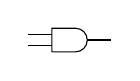
\begin{tikzpicture}[scale=0.3]
                                    \draw (0,0) -- (0,1) -- (1,1) arc (90:-90:0.5) -- (0,0);
                                    \draw (-1,0.25) -- (0,0.25);
                                    \draw (-1,0.75) -- (0,0.75);
                                    \draw (1.5,0.5) -- (2.5,0.5);
                                    \end{tikzpicture} \\
                                    \hline
                                    $p \vee q$ & p or q & 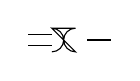
\begin{tikzpicture}[scale=0.3]
                                    \draw (0,0) arc (-90:90:0.5) -- (1,0) arc (270:90:0.5) -- (0,1);
                                    \draw (-1,0.25) -- (0,0.25);
                                    \draw (-1,0.75) -- (0,0.75);
                                    \draw (1.5,0.5) -- (2.5,0.5);
                                    \end{tikzpicture} \\
                                    \hline
                                    $\sim p$ & not p & \begin{tikzpicture}[scale=0.3]
                                    \draw (0,0.5) -- (1,0.5);
                                    \draw (1,0.5) circle (0.3);
                                    \draw (1.3,0.5) -- (2.3,0.5);
                                    \end{tikzpicture} \\
                                    \hline
                                    \end{tabular}
                                    \end{center}
                                    \end{frame}
                                    
                                    \begin{frame}
                                    \frametitle{Review: Putting It All Together}
                                    \begin{itemize}
                                        \item Propositional logic provides tools for analyzing the structure of arguments.
                                        \item We use symbols ($\sim$, $\wedge$, $\vee$, $\rightarrow$, $\leftrightarrow$) to represent logical operations.
                                        \item Truth tables help us determine when complex statements are true or false.
                                        \item Valid argument forms like modus ponens and modus tollens allow us to draw correct conclusions.
                                    \end{itemize}
                                    
                                    \begin{alertblock}{Key Takeaways}
                                        \scriptsize
                                    \begin{itemize}
                                        \item Learn to recognize logical patterns in everyday language.
                                        \item Be wary of common fallacies like affirming the consequent and denying the antecedent.
                                        \item Use truth tables to analyze complex statements systematically.
                                        \item Remember that logical validity is about the form of an argument, not its content.
                                        \item Propositional logic is the foundation for more advanced logical systems.
                                    \end{itemize}
                                    \end{alertblock}
                                    \end{frame}
\end{document}